\begin{center}
    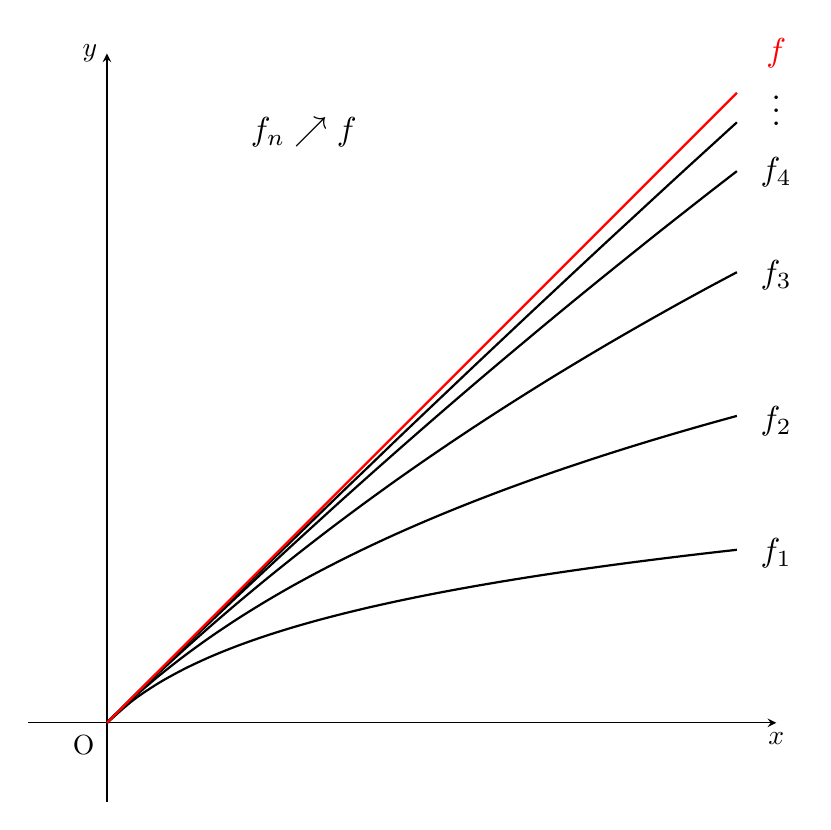
\begin{tikzpicture}
        \node[below left=1pt] (origin) at (0,0) {\(\rm{O}\)};
        \draw [-stealth] (-1, 0) -- (8.5, 0) node[below] {\(x\)};
        \draw [-stealth] (0, -1) -- (0, 8.5) node[left] {\(y\)};

        \foreach \n in {1, 3, 9, 27, 81} {
            \draw[thick, domain=0:8, smooth, variable=\x] plot ({\x}, {\n * ln(1 + \x / \n)});
        }
        \foreach \n in {1, 2, 3, 4} {
            \node[scale=1.2] at (8.5, {(3 ^ (\n - 1)) * ln(1 + 8.5 / (3 ^ (\n - 1))) - 0.1 * \n}) {\(f_{\n}\)};
        }
        \draw[thick, domain=0:8, smooth, variable=\x, color=red] plot ({\x}, {\x});
        \node[scale=1.2] at (8.5, 7.9) {\(\vdots\)};
        \node[scale=1.2, color=red] at (8.5, 8.5) {\(f\)};

        \node[scale=1.2] at (2.5, 7.5) {\(f_n \nearrow f\)};
    \end{tikzpicture}
\end{center}

\section*{Convergence Theorems}

르벡 적분 이론에서 굉장히 자주 사용되는 수렴 정리에 대해 다루겠습니다. 이 정리들을 사용하면 굉장히 유용한 결과를 쉽게 얻을 수 있습니다.

먼저 단조 수렴 정리(monotone convergence theorem, MCT)입니다. 이 정리에서는 \(f_n \geq 0\) 인 것이 매우 중요합니다.

\thm{11.28} \note{단조 수렴 정리} \(f_n: X \ra [0, \infty]\) 가 measurable이고 모든 \(x \in X\) 에 대하여 \(f_n(x) \leq f_{n+1}(x)\) 라 하자. \[
    \lim_{n\ra\infty} f_n(x) = \sup_{n} f_n(x) = f(x)
\]
로 두면,
\[
    \int f \d{\mu} = \lim_{n\ra\infty} \int f_n \d{\mu} = \sup_{n \in \N} \int f_n \d{\mu}
\]
이다.

\pf \\
\note{\(\geq\)} \(f_n(x) \leq f(x)\) 이므로 단조성을 이용하면 모든 \(n \in \N\) 에 대하여 \(\ds \int f_n \d{\mu} \leq \ds \int f \d{\mu}\) 이다. 따라서 다음이 성립한다.
\[
    \sup_n \int f_n \d{\mu} \leq \int f \d{\mu}.
\]

\note{\(\leq\)} 실수 \(c \in (0, 1)\) 를 잡자. 마지막에 \(c \nearrow 1\) 로 둘 것이다. 이제 measurable simple function \(s\)가 \(0 \leq s \leq f\) 라 하자. 그러면 모든 \(x \in X\) 에 대하여 \(c \cdot s(x) < f(x)\) 일 것이다.

이제
\[
    E_n = \{x \in X : f_n(x) \geq cs(x)\}
\]
으로 두면, \(f_n(x) - cs(x)\) 가 measurable function이므로 \(E_n\) 또한 measurable이다. 여기서 \(f_n\)이 증가하므로 \(E_n\subset E_{n+1} \subset \cdots\) 임을 알 수 있고 \(f_n \ra f\) 이므로 \(\bigcup_{n=1}^\infty E_n = X\) 이다.

충분히 큰 \(N \in \N\) 에 대하여 \(n \geq N\) 일 때, 모든 \(x\)에 대하여 \(f(x) \geq f_n(x) > cs(x)\) 가 되게 할 수 있다. 그리고 \(f_n \geq f_n \chi_{E_n} \geq cs \chi_{E_n}\) 이므로
\[ \tag{\mstar}
    \int f_n \d{\mu} \geq \int f_n \chi_{E_n} \d{\mu} \geq c\int s \chi_{E_n} \d{\mu},
\]
이고 여기서 \(s, \chi_{E_n}\)는 simple function이다. 그러므로 \(s = \sum_{k=0}^m y_k \chi_{A_k}\) 라고 적으면
\[
    s\chi_{E_n} = \sum_{k=0}^m y_k \chi_{A_k\cap E_n} \implies \int s \chi_{E_n} \d{\mu} = \sum_{k=0}^m y_k \mu(A_k\cap E_n)
\]
이다. \(n\ra\infty\) 일 때 \(A_k\cap E_n \nearrow A_k\) 이므로, continuity of measure를 사용해 \(\mu(A_k \cap E_n) \nearrow \mu(A_k)\) 를 얻고
\[
    \lim_{n\ra\infty} \int s \chi_{E_n}\d{\mu} = \int s \d{\mu}
\]
임도 알 수 있다. 이제 (\mstar)를 이용하면
\[
    \lim_{n\ra\infty} \int f_n \d{\mu} \geq c\int s \d{\mu}
\]
이므로, \(c \nearrow 1\) 로 두고 \(0\leq s\leq f\) 에 대하여 \(\sup\)을 취하면
\[
    \lim_{n\ra\infty} \int f_n \d{\mu} \geq \sup_{0\leq s\leq f} \int s \d{\mu} = \int f \d{\mu}
\]
가 되어 원하는 결과를 얻는다.

\rmk 만약 부등식 \(0 \leq f_n \leq f_{n+1}\) 이 정의역 전체가 아닌 정의역의 부분집합 \(E\)에서만 성립한다고 하면, 다음과 같이 생각할 수 있다.
\[
    0 \leq f_n \chi_E \leq f_{n+1} \chi_E \nearrow f \chi_E.
\]
그러므로 단조 수렴 정리가 \(E\)에서도 성립함을 알 수 있다.
\begin{center}
    \(E\)에서 \(0\leq f_n \leq f_{n+1} \nearrow f\) 이면 \(\ds \lim_{n\ra\infty} \int_E f_n \d{\mu} = \int_E f \d{\mu}\).
\end{center}

\rmk 함수열 \(f_n\)이 증가하는 경우에만 정리가 성립합니다. 감소하는 경우에는 반례로 함수 \(f_n = \chi_{[n, \infty)}\) 를 생각할 수 있습니다. 그러면 \(n \ra \infty\) 일 때 \(\chi_{[n, \infty)} \searrow 0\) 입니다.

그러면 Lebesgue measure \(m\)에 대하여
\[
    \infty = \int \chi_{[n, \infty)} \d{m} \neq \int 0 \d{m} = 0
\]
이 되어 단조 수렴 정리가 성립하지 않음을 확인할 수 있습니다.

\dots

지난 번에 \(f \geq 0\) 가 measurable이면 증가하는 measurable simple 함수열 \(s_n\)이 존재함을 보였고, 이 \(s_n\)에 대하여 적분값을 계산하여
\[
    \int_E s_n \d{\mu} = \sum_{i=1}^{n2^n} \frac{i - 1}{2^n}\mu\paren{\left\{x \in E : \frac{i-1}{2^n} \leq f(x) \leq \frac{i}{2^n}\right\}} + n\mu(\{x \in E : f(x)\geq n\})
\]
라는 결과까지 얻었습니다. 그런데 여기서
\[
    f(x) = \ds \lim_{n\ra\infty} s_n(x)
\]
이기 때문에, 단조 수렴 정리에 의해
\[
    \int_E f \d{\mu} = \lim_{n\ra\infty} \int_E s_n \d{\mu}
\]
가 성립하여 기대했던 결과를 얻었습니다. 지난 번 설명한 것처럼, 이는 곧 르벡 적분은 치역을 잘게 잘라 넓이를 계산한 것으로 이해할 수 있다는 의미가 됩니다.

\bigskip

다음은 단조 수렴 정리를 활용하여 유용한 결과를 쉽게 얻을 수 있는 예제입니다.

\rmk Measurable function \(f, g \geq 0\) 과 \(\alpha, \beta \in [0, \infty)\) 에 대하여 다음이 성립한다.
\[
    \int_E \paren{\alpha f + \beta g} \d{\mu} = \alpha \int_E f \d{\mu} + \beta \int_E g\d{\mu}.
\]

\pf Measurable function은 measurable simple function으로 근사할 수 있고, \(f, g \geq 0\) 이므로 단조증가하도록 잡을 수 있다. 그러므로 measurable simple function \(f_n\), \(g_n\)에 대하여 \(0 \leq f_n \leq f_{n+1} \nearrow f\), \(0 \leq g_n \leq g_{n+1} \nearrow g\) 으로 잡는다.

그러면 \(\alpha f_n + \beta g_n \nearrow \alpha f + \beta g\) 이고 \(\alpha f_n + \beta g_n\) 은 단조증가하는 measurable simple 함수열이다. 따라서 단조 수렴 정리에 의해
\[
    \int_E \paren{\alpha f_n + \beta g_n} \d{\mu} = \alpha \int_E f_n \d{\mu} + \beta \int_E g_n \d{\mu} \ra \alpha \int_E f \d{\mu} + \beta \int_E g\d{\mu}
\]
이다.

이와 비슷한 방법을 급수에도 적용할 수 있습니다.

\thm{11.30} Measurable function \(f_n: X \ra [0, \infty]\) 에 대하여 \(\sum_{n=1}^\infty f_n\)는 measurable이고, 단조 수렴 정리에 의해 다음이 성립한다.
\[
    \int_E \sum_{n=1}^\infty f_n \d{\mu} = \sum_{n=1}^\infty \int_E f_n \d{\mu}.
\]

\pf \(\sum_{n=1}^\infty f_n\)는 measurable function의 극한이므로 measurable이다. 무한급수를 부분합의 극한으로 생각하면 \(f_n \geq 0\) 이므로 부분합이 증가함을 알 수 있다. 따라서 단조 수렴 정리를 적용하여 결론을 얻는다.

\dots

단조 수렴 정리와 동치인 수렴 정리를 하나 더 소개합니다. Fatou lemma로 알려져 있습니다.

\thm{11.31} \note{Fatou} \(f_n \geq 0\) 가 measurable이고 \(E\)가 measurable이라 하자. 다음이 성립한다.
\[
    \int_E \liminf_{n\ra\infty} f_n \d{\mu} \leq \liminf_{n\ra\infty} \int_E f_n \d{\mu}.
\]

\pf \(g_n = \ds \inf_{k \geq n} f_k\) 으로 두면 \(\ds \lim_{n \ra \infty} g_n = \liminf_{n\ra\infty} f_n\) 이다. \(g_n\)이 증가함은 쉽게 확인할 수 있으며 \(g_n \geq 0\) 이다. \(g_n\)의 정의로부터 모든 \(k \geq n\) 에 대하여 \(g_n \leq f_k\) 이므로,
\[
    \int_E g_n \d{\mu} \leq \inf_{k\geq n} \int_E f_k \d{\mu}
\]
이다. 여기서 \(n \ra \infty\) 로 두면
\[
    \int_E \liminf_{n\ra\infty} f_n \d{\mu} = \lim_{n \ra \infty} \int_E g_n \d{\mu} \leq \lim_{n \ra \infty} \inf_{k \geq n}\int_E f_k \d{\mu} = \liminf_{n \ra \infty} \int_E f_n \d{\mu}
\]
이 된다. 여기서 첫 번째 등호는 단조 수렴 정리에 의해 성립한다.

\rmk 위 증명에서는 단조 수렴 정리를 활용했습니다. 반대로 이 정리를 가정하면 단조 수렴 정리를 증명할 수 있기도 합니다. 따라서 이 둘은 동치입니다. 증명은 생략합니다.

\rmk 왠지 위와 비슷한 결론이 \(\limsup\)에 대해서도 성립해야 할 것 같습니다. 구체적으로,
\[
    \int_E \limsup_{n \ra \infty} f_n \d{\mu} \geq \limsup_{n \ra \infty} \int_E f_n \d{\mu}
\]
일 것 같습니다. 안타깝게도 이는 성립하지 않습니다. 반례로 앞서 소개한 \(\chi_{[n, \infty)}\)를 한 번 더 가져올 수 있습니다. 좌변을 계산해 보면 0이지만, 우변을 계산해 보면 \(\infty\)입니다. 나중에 소개하겠지만, \(\abs{f_n} \leq g\) 를 만족하는 함수 \(g \in \mc{L}^{1}\) 가 존재해야 위 부등식이 성립합니다.

\rmk 르벡 적분의 몇 가지 성질을 소개하고 마칩니다.
\begin{enumerate}
    \item \(f\)가 measurable이고 \(E\)에서 bounded이며 \(\mu(E) < \infty\) 일 때, 적당한 실수 \(M > 0\) 에 대하여 \(\abs{f} \leq M\) 이므로
          \[
              \int_E \abs{f} \d{\mu} \leq \int_E M \d{\mu} = M\mu(E) < \infty
          \]
          임을 알 수 있습니다. 그러므로 \(f \in \mc{L}^{1}(E, \mu)\) 입니다. \(E\)의 measure가 finite라는 가정 하에, bounded function은 모두 르벡 적분 가능합니다.

    \item \(f, g \in \mc{L}^{1}(E, \mu)\) 이고 \(E\)에서 \(f \leq g\) 일 때, 단조성이 성립함을 보이려고 합니다. 앞에서는 \(0 \leq f \leq g\) 인 경우에만 단조성을 증명했었는데, 이를 확장하여 함수가 음의 값을 가지는 경우에도 증명하고 싶습니다. 그러므로 양수인 부분과 음수인 부분을 나누어 고려하여 다음과 같이 적을 수 있습니다.
          \[
              \chi_E (x) f^+(x) \leq \chi_E(x) g^+(x), \qquad \chi_E(x) g^-(x) \leq \chi_E (x) f^-(x)
          \]
          이로부터
          \[
              \int_E f^+ \d{\mu} \leq \int_E g^+ \d{\mu} < \infty, \qquad \int_E g^- \d{\mu} \leq \int_E f^- \d{\mu} < \infty
          \]
          를 얻습니다. 따라서
          \[
              \int_E f\d{\mu} \leq \int_E g \d{\mu}
          \]
          가 성립하고, 함수가 음의 값을 가지는 경우에도 단조성이 성립함을 알 수 있습니다.

    \item \(f \in \mc{L}^{1}(E, \mu)\), \(c \in \R\) 라 하면 \(cf \in \mc{L}^{1}(E, \mu)\) 입니다. 왜냐하면
          \[
              \int_E \abs{c}\abs{f} \d{\mu} = \abs{c} \int_E \abs{f}\d{\mu} < \infty
          \]
          이기 때문입니다. 적분이 가능하니 실제 적분값을 계산할 때 선형성이 성립했으면 좋겠습니다. 앞에서는 음이 아닌 실수에 대해서만 증명했었는데, 이도 마찬가지로 확장하려 합니다. \(c < 0\) 인 경우만 보이면 됩니다. 이 때, \((cf)^+ = -cf^-\), \((cf)^- = -cf^+\) 이므로, 다음이 성립합니다.
          \[
              \int_E cf \d{\mu} = \int_E (cf)^+ - \int_E (cf)^- \d{\mu} = -c \int_E f^- \d{\mu} - (-c) \int_E f^+ \d{\mu} = c\int_E f\d{\mu}.
          \]

    \item Measurable function \(f\)에 대하여 \(E\)에서 \(a \leq f(x) \leq b\) 이고 \(\mu(E) < \infty\) 일 때 다음이 성립합니다.
          \[
              \int_E a \chi_E \d{\mu} \leq \int_E f\chi_E \d{\mu} \leq \int_E b \chi_E \d{\mu} \implies a \mu(E) \leq \int_E f \d{\mu} \leq b \mu(E).
          \]
          \(f\)가 르벡 적분 가능하다는 사실은 \(f\)가 bounded라는 사실을 이용합니다.

    \item \(f \in \mc{L}^{1}(E, \mu)\) 와 measurable set \(A \subset E\) 가 주어지는 경우, \(f\)는 \(E\)의 부분집합인 \(A\) 위에서도 르벡 적분 가능합니다. 이는 다음 부등식에서 확인할 수 있습니다.
          \[
              \int_A \abs{f} \d{\mu} \leq \int_E \abs{f}\d{\mu} < \infty.
          \]

    \item 만약 measure가 0인 집합에서 적분을 하면 어떻게 될까요? \(\mu(E) = 0\) 라 하고, measurable function \(f\)를 적분해 보겠습니다. 여기서 \(\min\{\abs{f}, n\}\chi_E\) 도 measurable이며 \(n \ra \infty\) 일 때 \(\min\{\abs{f}, n\}\chi_E \nearrow \abs{f}\chi_E\) 임을 이용합니다. 마지막으로 단조 수렴 정리를 적용하면
          \[
              \begin{aligned}
                \int_E \abs{f} \d{\mu} &= \lim_{n \ra \infty} \int_E \min\{\abs{f}, n\} \d{\mu} \\
                &\leq \lim_{n \ra \infty} \int_E n \d{\mu} = \lim_{n \ra \infty} n\mu(E) = 0
              \end{aligned}
          \]
          임을 얻습니다. 따라서 \(f \in \mc{L}^{1}(E, \mu)\) 이고, \(\ds \int_E f \d{\mu} = 0\) 가 되어 적분값이 0임을 알 수 있습니다. 즉, measure가 0인 집합 위에서 적분하면 그 결과는 0이 됩니다.\footnote{편의상 \(0\cdot\infty = 0\) 으로 정의했기 때문에 \(f \equiv \infty\) 인 경우에도 성립합니다.}
\end{enumerate}

다음 글에서는 르벡 수렴 정리를 소개하겠습니다.

\pagebreak
